\newpage
\section{Experiments}

% 1) Very quick summary of the modelling tasks
% goal: use 2 types of tasks - graph classif and node regression
%       try some of the models
%       find a novel solution to a problem
% organization: the tasks selected are G-N approximation and  
The goal of this master's thesis is to apply Graph Neural Network models to different problems to create a novel solution. The idea is to get to know how Graph Neural Networks are used in each situation. Two problems are explored: Girvan-Newman algorithm approximation and compiled code function classification. They correspond to the two main tasks that Graph Neural Network perform with success, semi-supervised learning of nodes on a graph and supervised graph classification. 

This section will present the configuration of the experiments performed in the thesis. First, the Girvan-Newman approximation experiment is explained. Then the compiled code function classification experiment is described last. In each case, context, goals and motivation are described first. Then a preliminary test is performed on well-known benchmark datasets to verify the software libraries and setup in use work correctly in the computer without any problem. Then the process of data preparation is explained and finally how the part of training a model is executed is summarized.

% 2) Girvan-Newman approximation
\subsection{Girvan-Newman algorithm approximation}


\subsubsection{Experiment overview}

% 2.1) Girvan-Newman: description (review state of the art quickly),
\textbf{Context} \\
The Girvan-Newman algorithm is a clustering based approach to perform community detection. It proposed a divisive algorithm based on edge-betweenness for a graph with undirected and unweighted edges. The algorithm focused on edges that are most "between" the communities and communities are constructed progressively by removing these edges from the original graph. It iteratively isolates groups of nodes of a graph by removing the edges that poses the greater edge betweenness value. The worst-case for time complexity of the edge-betweenness algorithm is $O(m^2n)$ and is $O(n^3)$ for sparse graphs, with $m$ being the number of edges and $n$ the number of vertices. 

\textbf{Goal}\\
%          goal (approximate it), 
The goal of this experiment is to find a novel way to approximate the Girvan-Newman algorithm that is faster than the original.


\textbf{Motivation}\\
% motivation find a good balance point between speed and accuracy, 
Community detection is a popular task with applications in many areas related to social network analysis. An approximated but faster implementation could impact on tasks that need to detect community on large graphs, like the ones extracted from social networks, citation networks, and the like.


\textbf{Experiment}\\
%actual ideas for approximation
To be more precise, the function to approximate will be the computation of the edge betweenness for each edge of the graph in each iteration of the algorithm. Thus, the experiments will focus solely on finding a Graph Neural Network that approximates the computation of the edge betweenness of all edges of a graph with a reasonable performance.

% edge betweenness definition
For any node in a graph, node betweenness is defined as the number of shortest paths between pairs of nodes that run through it. The Girvan–Newman algorithm extends this definition to the case of edges, defining the "edge betweenness" of an edge as the number of shortest paths between pairs of nodes that run along it. If there is more than one shortest path between a pair of nodes, each path is assigned equal weight such that the total weight of all of the paths is equal to unity.

There are two main ways to approximate the edge betweenness with Graph Neural Network models. 

The first one, using supervised learning for doing edge attribute value regression. A model will be trained to approximate the edge betweenness of all edges of a graph. The final approximated Girvan-Newman algorithm would consist of the original process but replacing the computation of the edge betweenness by the trained model.


%               1) approxima edge_betweenness of all the nodes in each iteration of GN
% 				2) in each iteration, compute edge -betweenns of some nodes, then use GCN in a transductive setting to expand to the rest of nodes(hopefully faster)
The second approach, by using semi-supervised learning, one can compute the edge betweenness of several nodes and then train the model to predict the value for the rest of edges of the graph. In that case, the Girvan-Newman algorithm would, in each iteration, first compute the edge betweenness of some edges in the normal way, then use the model to approximate the edge betweenness of the rest of the edges of the graph. By the nature of the Graph Neural Networks that have attained state-of-the-art performance on semi-supervised learning, the second approach seems the most realistic one.

The give a bit more of context on the second approach to approximate the Girvan-Newman algorithm, the steps would be the following:
\begin{itemize}
	\item \textbf{1. Compute the edge betweenness of some edges of the graph:} One advantage is that we could limit how many edge betweenness's are computed by time. Let's say we allow for 10 seconds edge betweenness computations.
	\item \textbf{2. Approximate the edge betweenness of the rest of edges of the graph:} this steps would use a Gran Neural Network in a semi-supervised and transductive setting. This means that the Graph Neural Network should be trained on the actual graph or similar graphs before using it. It could also have another implication, that the graph neural network training can benefit from having a representative sample of the total population of edge betweennesses of the graph. However, this can only be approximated with some heuristic. For example, one could use for training several edges connected to nodes with a high degree and several edges connected to nodes with a low degree.
	\item \textbf{3. Selection of the most central edge:} this step would gather all edge betweenness values from previous steps and decide which edge to remove from the graph(the one with maximum edge betweenness). The rest of steps of the algorithm would go unchanged.
\end{itemize}




\subsubsection{Preliminary test}

As a way to verify that available code from published research works correctly on computer on which the experiments will be performed, a published experiment is reproduced. A task of semi-supervised classification is reproduced locally, training a set of GCN, ChebNet, GAT , SG and APPNP models. The Cora dataset is used for this task.  The Cora dataset(\cite{sen2008collective} consists of 2708 scientific publications classified into one of seven classes. The goal is to verify that the computer that will support the experiments can train those models without memory problems or other types of problems. Also it is a way to check that some configurations of hyper-parameters yield good results for later comparison with the real experiments. 


% 2.2) data gathering process
\subsubsection{Dataset}


\textbf{Datasets used}\\
%  collection process(Pytorch Geometric dataloader)
%  types of graphs used
For the Girvan-Newman aproximation experiment, well known datasets available from Pytorch Geometric library are considered and inspected:
\begin{itemize}
	\item Cora
	\item Watts-Strogatz random generated graph,
	\item and Karate-Club.
\end{itemize}
From all of the graphs in those databases, the ones that show a larger number of nodes and higher edge betweennesses values, with the contraints of the memory limit of the computer used, are selected. The reason is the following, for training a model for predicting the edge betweenness of an edge, some parts of a graph are used as training, validation and others as testing. This implies that a small graph will produce dataset splits that contain few edges and so the model trained on those small subgraphs usually won't be able to learn a good approximation. In the testing and inspection of the graphs, the datasets that contain several small graphs are treated as a big graph with disconnected components. When the dataset contains only one graph, it will usually be big and so the sub graphs splits for training, validation and testing will be enough in size for the model to train properly. The final selection has been to use the CORA dataset. %a Watts-Strogatz with 100 nodes and the Karate-Club graph.



\textbf{Data preparation}
%  data inspection(None)
%  precomputation of the edge-betweennes for target preparation

The first step in data preparation is to compute the actual edge betweenness of each edge of the graph, and save all those in the target (or ground true) vector. To compute the edge betweenness, the Python library NetworkX is used. First, the graph is transformed from the Pytorch Geometric Dataset format to a list of edges on a file on disk. This list of edge is then read by the NetworkX library to transform it into a NetworkX graph object. Then, the edge betweenness function of NetworkX is called. The result is a dictionary (key-value map) with the edge betweenness of each edge.


The setup of the target value, the ground truth value of the edge betweenness of each edge of the graph, will be specific to how the graphs of a dataset are handled. When there's only a graph on the dataset, it is straight forward to compute the edge betweenness of each edge from the NetworkX graph library and used it as the ground truth(the target value) for the model training. When the dataset contains many separated graphs, there are two ways to approach the experiment. The first way is to process all graphs together as if it was a big graph with disconnected components and compute the edge betweenness in this setup. The second way is to process all graphs together as a big graph with connected components but to compute the edge betweenness for each graph alone. We will limit the experiment to big unique graphs without unconnected parts.


There are two ways to train a model for the edge betweenness. One way is to do a regression on the value of the edge betweenness, in which case the performance metric would be the normalized root mean squared error. The other way is to group edge betweenness values into groups (or buckets) and then consider each group a class, to be able to train a classification model. In this second way the performance metric will be the accuracy. The classification approach has yielded better results and so is the one selected. For creating the buckets or groups, a series of limit values are chosen, then an histogram of counts for each class is generated. This step is repeated until the histogram shows there is a small class imbalance(all histogram bars are almost same size). Finally, the information of the limits of the buckets allows us to transform the vector with true edge betwenness real values into the number of the bucket they belong to. Thus, this number will be the class or group identifier, that the classifier will learn to predict. For the algorithm to work correctly, the class numbers are assigned from 0 to the number of classes minus 1.

%The training, validation and testing split of edges of the graph has a big impact on the final model performance. The reason is that, training the model on edges that have only a small range of edge betweennesses will likely produce a model less unable to generalize to unseen edges. So the nodes/edges splits have to be chosen carefully. One idea is to produce splits that contain representative samples of the values of the edge betweennesses of all the graph. One way to verify a split is correct is to compute summary statistics of the edge betweenness values of each split and compare, with a box plot, that they are all similar. If they are all similar, as seen in left plot of \ref{fig:edgeb_boxplot} it means each one of them has a population of edge betweennesses that is representative enough. 



% \begin{figure}[H]
% \minipage{0.5\textwidth}%
%   \centering
%     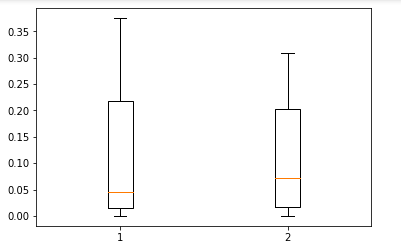
\includegraphics[width=0.9\linewidth]{img/graph_splits_boxplot.png}
% \endminipage
% \minipage{0.5\textwidth}%
%   \centering
%     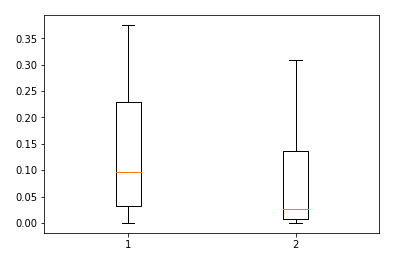
\includegraphics[width=0.9\linewidth]{img/graph_splits_boxplot2.png}
% \endminipage
% \caption{Boxplots of the values of the edge betweenness in 2 different dataset splits}\label{fig:edgeb_boxplot}
% \end{figure}

%The final dataset preparation is therefore to find good dataset splits for training, validation and testing. A quick way to find those splits, is to fix the randomness of the dataset sampling mechanism with a seed and explore which seed value satisfies the properties we want from our dataset splits. The exploration is simply done by incrementing sequentially the seed, then for each seed value computing the dataset split, then computing a measure of dissimilarity between the values of edge betweennesses of each split. In that particular case, the splits have the same size, the edge betweennesses values are sorted in each split, and a mean squared error is computed  from each pair of values from each split in order. The mean squared error is computed first between train and testing split and then between train and validation split and the errors are summed. The seed that obtain a lower error are the ones used in the training.

For the setup of the dataset splits, the approach has been to generate small sized training splits, and middle and large sized validation and testing splits. This is to satisfy the semi-supervised learning transductive setting. The total number of edges of the graph is divided in 3 different sizes, after applying some random permutation. The size of the training split is computed as the number of classes time a low number like 20 or 300 depending on the size of the graph. The rest of edges are divided into validation and testing split, with a proportion of 1 to 3 or 1 to 1. 




\subsubsection{Model training}
% 2.3) Experiments list (main task and side analysis)
%  GCN training
%  graphSage training

Since the dataset splits could have a high impact on the performance of the trained model, each training is repeated a number of times, for instance 100 times, and the performance is averaged over all the repetitions. This averaging process would compensate for when a very unbalanced dataset split is generated and a model trained on it.


 The type of model used is one that allows us to update the state of the edge attributes in the aggregation and combine phase of the iterative process. PyTorch Geometric python library implements a Message Passing Neural Network \cite{mpnn} that is highly generalizable, called MetaLayer (see \cite{battaglia2018relational} and \cite{fey2019fast} ), that allows for updating edge attributes. Based on this architecture, different adjustments on the number of layers, the number of units of layers, and other hyper parameters will be modified during hyper-parameter search. 



\begin{figure}[H]
    \centering
        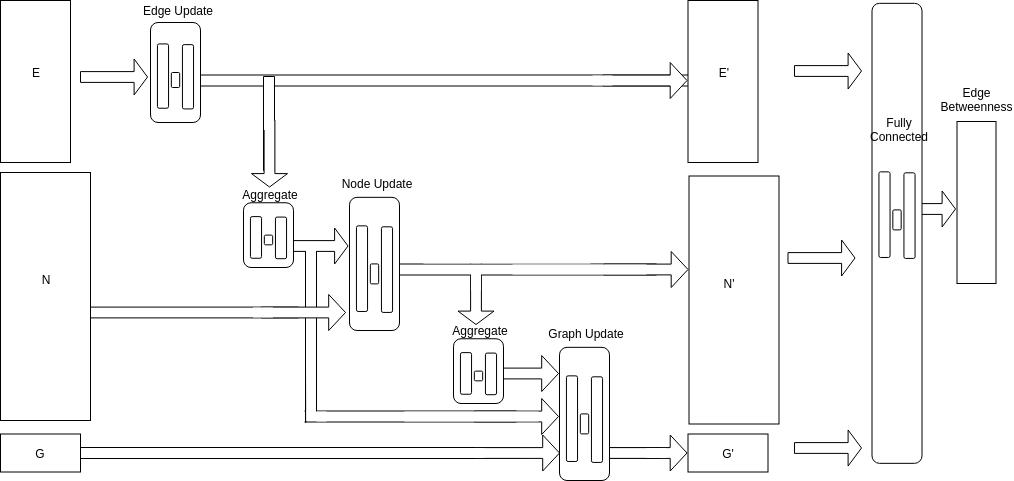
\includegraphics[width=0.85\linewidth]{img/GN_exp1_metalayer2.png}
    \caption{Architecture of the MetaLayer model}\label{fig:metalayer_diagram}
\end{figure}

 The architecture of the MetaLayer model is composed of 4 building blocks. First the node states(also called attributes or features), the edge states and the graph level state are concatenated and fed to the first block: the edge multilayer perceptron(MLP). The edge MLP is a 2 layer neural network with a ReLU in between. The next step is to aggregate the output of the edge MLP per node, concatenate it to the node and graph states and feed this to the node MLP. This second block has 2 MLP networks, one for the aggregation and the other for the combination, each one with 2 layer neural network with a ReLU activation unit in between. Then the edges attributes and node attributes are aggregated globally and the global state of the graph is updated. The output of the MetaLayer is an identical graph with the states (attributes) updated. This new graph stats is fed to 2 fully connected layers that will produce the final edge attributes. The number of units in each layer can be controlled as parameters, which are optimized in an hyper parameter search. Actually this hyper parameter search could be made much more intensive. In this experiment, we don't use the graph level state and graph level state update.

 \begin{figure}[H]
    \centering
        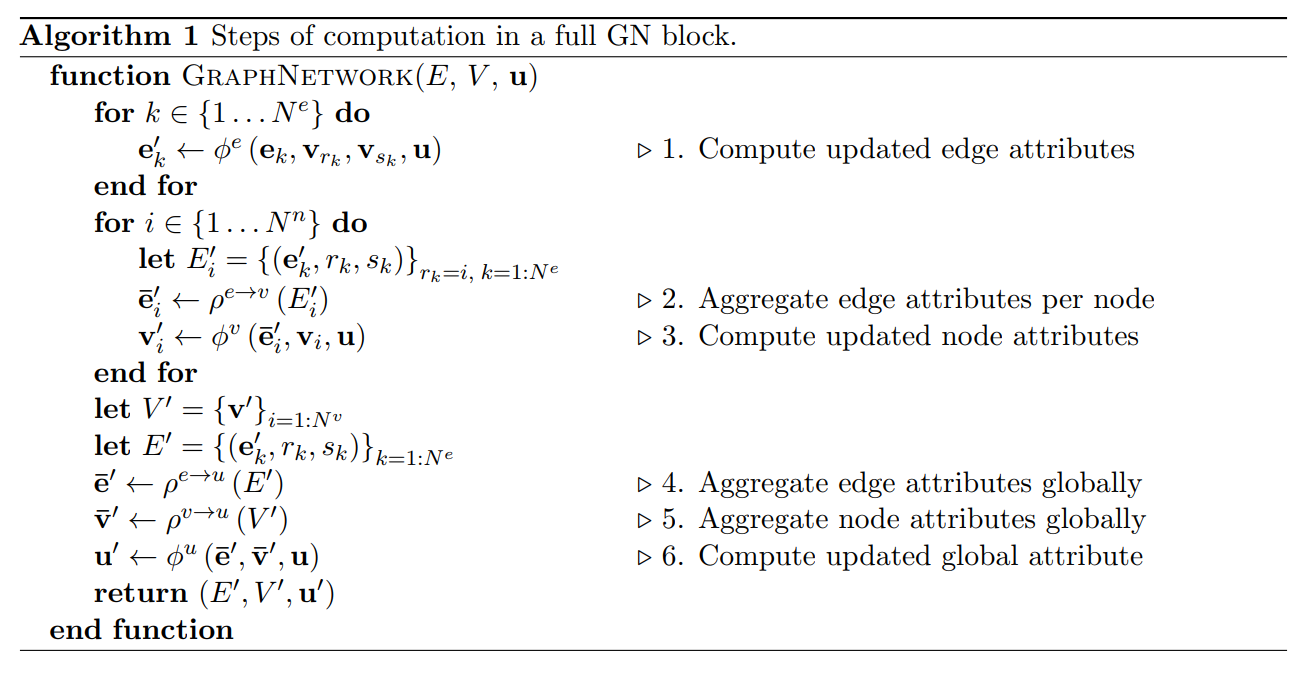
\includegraphics[width=0.85\linewidth]{img/metalayer-algorithm.png}
    \caption{Architecture of the MetaLayer model (Battaglia et al. 2018  \cite{battaglia2018relational} )}\label{fig:metalayer_algorithm}
\end{figure}

%If this experiment does not attain an acceptable performance, it will be modified into approximate other graph measures like node betweenness centrality or PageRank. An important point to stress here is that spatial based graph convolutional method have a limitation on the sensibility to long range relationships.  There is a spectral based graph convolutional method available, but it's only applicable to node features. This will consequently be tested, to try to see if long range relationship visibility increases with these types of models


%A complementary experiment performed is to try to approximate other centrality measures from a graph. Betweenness centrality(for nodes) and PageRank have been used to train models to approximate them. The types of models include GCN, GraphSage and the spectral-based ChebNet \cite{}defferrard2016convolutional}.

\textbf{Evaluation procedure}\\
%  inspecting the distribution of results
To evaluate the results, the performance metric used is the accuracy. We could use the F1-score in macro or micro averages, but since the bucketization process is intented to remove class imbalance, the accuracy is still valid.


As a complement to understand how much performance a model attains, the distribution of predicted values versus their true target values is compared in a scatter plot. The cloud of points is plotted in the 2D, to be able to see if it deviates from the 45º line (y=x line). An histogram and a boxplot are also used to inspect the distribution of predicted values versus the target values. All of them are compared with the target values in buckets and also compared with the real values of the edge betweenness \\
\\



\newpage
\subsection{Compiled code function classification}
% 3) Function renaming

\subsubsection{Experiment overview}

\textbf{Context}
% 3.1) Function renaming: 
%  description: quick recap of sota about code2vec and varnaming tasks

There have been some research publications related to the topic of program analysis. As mentioned in the section 2, there have been approaches to classify code snippets \cite{code2vec} and variables \cite{139} and their usage so that a name can be assigned to them. 

\textbf{Goal}

%  goal: apply those same tasks to compile code (assembler)
Inspired by those examples, the second experiment of this thesis tries to create a predictive model that will classify a snippet of code in assembler language, the programming language that has a direct transcription to machine code in compiled binaries. The experiment will focus on entire functions or subroutines in assembler language. The experiment will not try to replicate any of the conditions of the research that inspired it, since this experiment will be performed on a different programming language than \cite{139} and \cite{code2vec} and a different kind of model than \cite{code2vec}.

\textbf{Motivation}
%  motivation: reverse engineering for malware(malicious code) analysis (process steps, where the algorithm could help)
%              what is the decision on the precise goal: main functionalities(crypto, network, disk, ..)

This experiment could build a classification model that is useful for professionals that work on anti-virus companies. In any anti-virus company, there are security engineers that analyze malicious code, also called computer virus or malware. Part of the process of analyzing a malicious code consists in reverse engineering the code contained inside a binary file. Besides fighting against code obfuscation techniques, the reverse engineer is faced with several thousands of assembler subroutines or functions that he needs to inspect to find where the important code functionalities reside. One way to proceed is from the hints of the interaction of the malicious code with its environment. When a malicious code reads files or connects to Internet urls, called artifacts, the reverse engineer can begin to trace back the functions that use those artifacts. In the process of tracing the code related to those artifacts, or in looking for main actions like connection to the Internet, the reverse engineer will write comments, annotate code snippets or rename functions.
It is estimated that having an indication of the main functionality that a code snippet performs can help reverse engineers to find more quickly the evidences they need when analyzing malicious code. This indication can be implemented as renaming the functions of a binary. The renaming of a function can be based on the classification that a machine learning model will predict on it.



\textbf{Experiment}
%  overview of the process: building the dataset, transform it, label it, preprocessing, then training the models

The experiment consists in several complex steps.
First, building a dataset that is suitable for training a model on classifying code on a set of predefined classes. Some binaries that contain functions related to the chosen predefined classes are collected from open source software.  
Next, those binaries and their functions are analyzed by a program that translates machine code to assembler language. This kind of tool is called a disassembler.
Then, different representations of those functions in assembler have to be generated: a graph for each function and some features related to the assembler code itself and to the structure of the graph.
After that, the collected dataset must be correctly labeled. Since the intent is to train a model in a supervised setting, each function (corresponding to a sample of the dataset) must be labeled with one of the predefined classes.
Finally, with the dataset correctly labeled and with all its features in place, the models can be trained to classify assembler code functions. A set of baseline classification models, then some basic NLP models and finally a set of GNN models will be trained. 

\subsubsection{Preliminary experiment}

A reproduction of some of the results in graph classification tasks by Graph Neural Networks are replicated in this project to make sure that we are able to attain a similar performance with the tools at hand (Pytorch implementation of Graph Neural Network components). The graph classification tasks on the datasets:
\begin{itemize} 	
	\item Proteins, 
	\item REDDIT binary
	\item and QM9 
\end{itemize} 

are reproduced with different model architectures than the ones on the benchmarks of Pytorch Geometric library. The results are based on the f1-macro average score.




\subsubsection{Dataset}
% 3.2) data gathering process

Let's first review the complex data preparation process. There's no open source dataset with the properties needed for the experiment so it will be created from scratch.



\textbf{Data sources}
% sources of compiled code: malware samples(why not?  unlabeled and on top of it obfuscated)
%                           well-known softare: webservers, cryptographic libraries, disk utilis,  copyright protection software

Since the main audience could be malicious software analysts, one possibility of getting data from would be to collect analyzed malicious code. It turns out that there's not many sources of analyzed malicious code, and also, malicious code is plenty of obfuscation techniques, which would be an entire different experiment to deal with. 

Instead, the preferred strategy is to use well-known software that contains the functionality according to the predefined classes. A decision was need to be made on the set of labels that the dataset will contain. A set of main functionalities related to general purpose applications would be:
\begin{itemize}
	\item network
	\item cryptography
	\item disk access
	\item memory manipulation
\end{itemize}
According to that list, several open source tools and libraries are collected, in order to have at least several binaries in each of the previous categories. To that end, open source binaries from web servers, email clients, ftp servers and clients, cryptographic libraries, disk utilities and C library are collected. The list of used software is detailed in the Annex \ref{annex:compilation}.

To be able to later assign a label to each sample, where each sample is a function from the selected applications, there are a few options available. The first one is to consider all functions of a binary to be labelled with the main purpose of the binary. For example, all functions of a web server would be labelled network. This approach is too coarse grained and therefore may lead to useless classification models. A second approach would consist in obtaining the open source software sources and then compiling it with debugging information. This type of compilation maintains the original function names that developers assigned to functions. Examples of function names are \textit{asn1\_print\_fsname} and \textit{bio\_sock\_error}(see Annex \ref{annex:compilation}).



\textbf{Data transformation}
% data transformation: plugin to extract assembly code as a graph. 

For generating the dataset, a plugin in Python programming language has been developed to be used inside a disassembler program, namely the free version of IDA (\href{https://www.hex-rays.com/products/ida/support/download\_freeware.shtml}{IDA Freeware version}), a popular professional disassembler program but in its freeware version. As introduced in the context of this experiment, a disassembler is a program that reads compiled binaries and converts machine instructions to assembler instructions, and its main purpose is to reverse engineer software for debugging purposes.


% abstract idea - each instruction/register/memaddr... is a node
% in which instruction it is used is a vertex
% 									  order of executions of instructions form vertex between then + branchs/calls/loops...
%									NetworkX format from txt files 
This plugin visits all the functions detected in a binary and extracts the information of instructions, operands and cross-references to generate a graph of the relationship between them. Every instruction, operand, memory address or constant is a node of the graph. Every relationship between them is a vertex of that graph. There's worth mentioning that instructions are executed one after another and so usually an instruction will be linked to its previous and next instruction in the execution flow. However, sometimes loops, conditional branches and function calls modify this sequential execution flow by adding extra edges.

The graph is saved in a format suitable for the Python library NetworkX to read it and import it. The format consists of 2 text files, one with the list of nodes and their attributes, the other with the list of edges and their attributes. For more details, see Annex \ref{annex:graph_from_code}.




\textbf{Supervised labels generation}
% 3.3) labelling discussion
		% approach1: all assembly code from a binary under the same label
		% approach2: compile with symbols and then infer label from function name
		%            rules: topics and tasks, 
		%            final sets of labels v1,v2,v3

After obtaining the assembler code of each functions and its original name, some simple rules where created to derive a label from the function name in a programatic way. Basically the appearance of keywords would drive this process. Additionally, human supervision has been applied to improve the labeling assignments. 

Four different versions of the dataset have been generated:
\begin{itemize}
	\item v0: each binary and all its functions have the same label. This is a coarse grained and unrealistic approach. It is suspected that the models would learn spurious relations with this dataset.
	\item v1: 10 different labels have been chosen, and function labels has been assigned by keyword appearance in the debugging information (original function name).
	\item v2: a list of topic and tasks has been compiled and combined to generate 120 different labels. Keyword appearance rules and human supervision have been used to assign labels.
	\item v3: a reduced list of topic and tasks has been compiled and combined to generate 24 different labels. Keyword appearance rules and human supervision have been used to assign labels.
\end{itemize}
The idea was to find the correct granularity of the dataset. Trained models tend to perform better in the smaller sets of labels (v0 and v1), but there is the risk that the model does not capture any of the information of interest. More detail can be found in Annex \ref{annex:labels}.





\textbf{Feature engineering}


% data transformation for baseline models: summary statistics of graphs, and other topological features
% data transformation for nlp models: Bag of words with TF-IDF
Besides the graph representation of each function of a binary file, the attributes that will be used by baseline models are also extracted or generated. There are topological features from the graphs and features extracted directly from the code itself, like the Bag of Words embedding (fined-tuned by TF-IDF). The topological features include the most common statistics on graph structure like diameter, average degree, average clustering, average shortest path length and assortativity coefficient. The code features, besides the Bag of words embedding from the words on the code itself, include number of registers, number of instructions, number of functions called, etc. The complete list can be found in the Annex \ref{annex:feature_engineering}.


\begin{figure}[H]
    \centering
        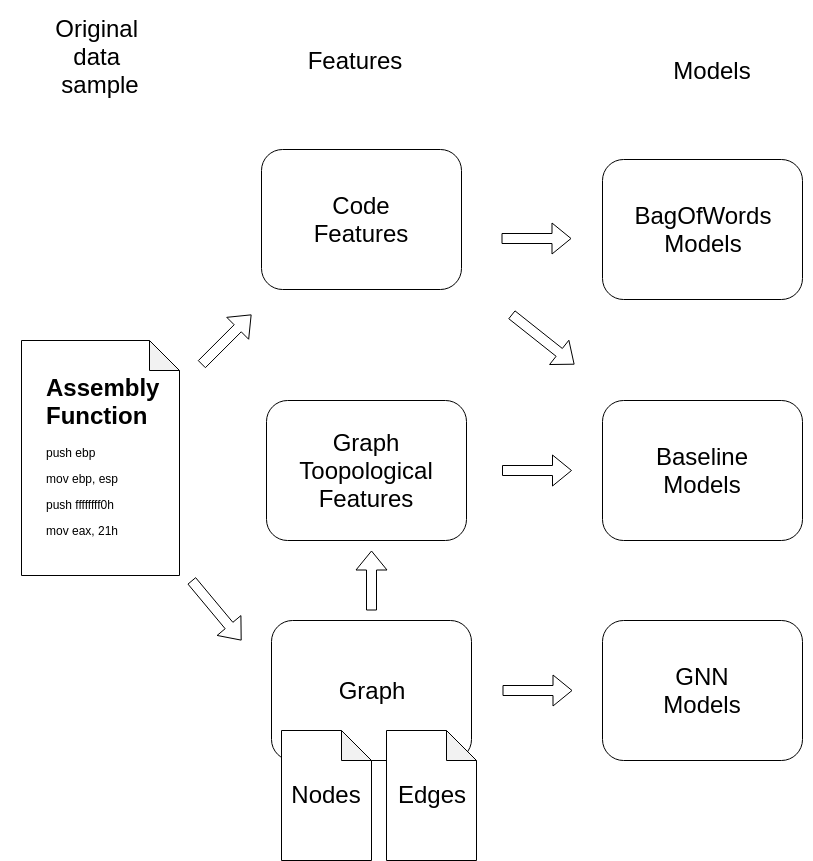
\includegraphics[width=0.55\linewidth]{img/Features_and_models_diagram.png}
    \caption{Features exracted from the dataset samples and their relationship with the models trained}\label{fig:Features_diagram}
\end{figure}

All of these features and graph representation will be transformed into a Dataset module from Pytorch Geometric library, \cite{fey2019fast}. This will allow the training of Graph Neural Network models to use the complete ecosystem of PyTorch Geometric for loading graphs, training models and test their performance. For the baseline models, the topological features and code features will be transformed into tensors of floats. And for the models that use bag of words embedding, the bag of words is not exactly generated in this stage, but it is rather fed by the string that contains all the code listing, during training time, to adjust the words to be taken into account by testing different maximum and minimum frequencies. Once the model is trained, it has also decided the best version of the bag of words embedding. In any case, the output of the bag of words is an embedding that is fed to the downstream machine learning models.

An initial distribution analysis is performed on the different code and topological features to see if the features carry any discriminative power within its signal. The analysis confirms there is a significant amount of signal in the data (\ref{annex:feature_engineering}).



\begin{figure}[H]
\minipage{0.5\textwidth}%
  \centering
    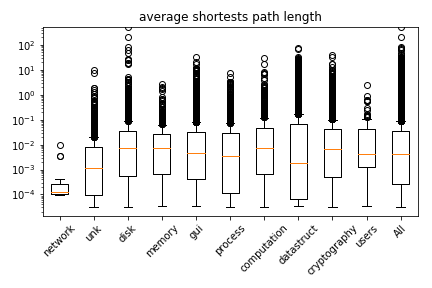
\includegraphics[width=0.9\linewidth]{img/boxplots/v1_unbalanced_average_shortests_path_length.png}
\endminipage
\minipage{0.5\textwidth}%
  \centering
    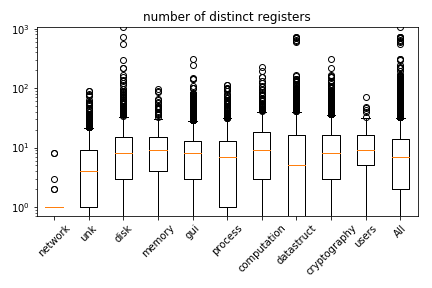
\includegraphics[width=0.9\linewidth]{img/boxplots/v1_unbalanced_number_of_distinct_registers.png}
\endminipage
\caption{Boxplots of the distribution of the data for several features}\label{fig:distribution_analysis}
\end{figure}





\subsubsection{Model training and evaluation}
% 3.4) Experiments list (each attempt with different datasets, baselines, nlp and ggnn)




\textbf{Compiled code classification models}
% function renaming experiments

% baseline models training (noisy,v1,v2,v3)
% nlp models training      (noisy,v1,v2,v3)
% gnn models training      (noisy,v1,v2,v3)

A set trainings will be performed on baseline models, Bag-of-word models and GNNs.

The set of baseline models used are:
\begin{itemize}
	\item Logistic Regression
	\item Decition trees
	\item Random Forest
	\item XGBoost
	\item MLP (Multi-layer perceptron)
\end{itemize}

The set of Bag-of-words models consists of the baseline models of the previous list, but using the bag-of-word tfidf embedding as an input. There will also be mixed features from topological features or code features, concatenated with the the Bag of words tfidf embedding.

The set of Graph Neural Networks used consists of combinations of:
\begin{itemize}
	\item pooling layers to reduce dimensionality
	\item GCN, GraphSage, Gated Graph Neural Networks, MetaLayer(Message Passing Neural Network) and Graph Isomorphism Network (GIN)
	\item global pooling to extract a graph level set of attributes
	\item some fully connected layers at the end
\end{itemize}

Based on this architecture, different adjustments on the number of layers, the number of units of layers, and other hyper parameters will be modified during hyper-parameter search.


\begin{figure}[H]
    \centering
        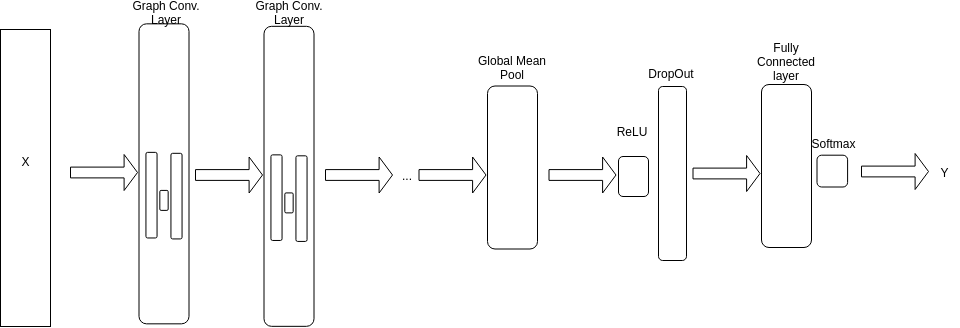
\includegraphics[width=0.85\linewidth]{img/GN_exp2_GIN.png}
    \caption{Architecture of the Graph Isomorphism Network (GIN) model}\label{fig:gin_diagram}
\end{figure}



\textbf{Evaluation}
To evaluate model performance, the f1-score with a macro average will be used. F1-score allows to measure precision and recall at the same time (it's the harmonic mean). To tackle the class imbalance present in the data, an undersample strategy on the training set has been applied to re-balance the classes, and then the Macro averages are used as the performance measure. Restoring class balance protects the training of the model from the possibility that it learns to classify only the majority class.
